% Part: sets-functions-relations
% Chapter: relations
% Section: trees

\documentclass[../../../include/open-logic-section]{subfiles}

\begin{document}

\olfileid{sfr}{rel}{tre}
\olsection{ونې}

د جزوي ترتيب يو خاص ډول چې د منطق په ټولو برخو کښې مهم رول لري،
\emph{ونه} ده۔ متناهي ونې د منطق په لومړنيو برخو کښې راځي:
مثلاً، !!{formula}s په نحوي ونه کښې د خپلو برخو په بېلولو پوهېدلے
شو، او په ډېرو !!{derivation} نظامونو کښې !!{derivation}s هم د
متناهي ونو بڼه خپلوي۔
%
نامتناهي ونې د بياني منطق او د لومړۍ درجې منطق د بشپړتيا د قضيو
په ثبوت کښې لا راڅرګندېږي، او په ټول رياضي منطق کښې کارول کېږي۔

د سټونو د نظريې د ونې مفهوم د ګرافونو په نظريه کښې د ونې له
مفهوم سره نژدې تړاو لري۔ دا د يوې (متناهي) ونې انځور دے:

\begin{center}
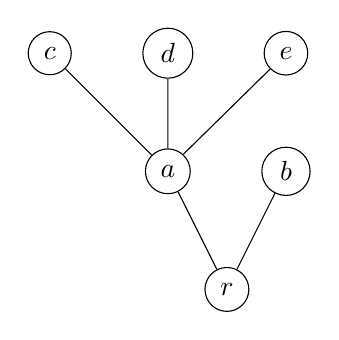
\begin{tikzpicture}[nodes={draw, circle}, -]
\node{$r$} [grow'=up]
    child { node {$a$}
        child { node {$c$} }
        child { node {$d$} }
        child { node {$e$} }
    }
    child { node {$b$} };
\end{tikzpicture}
\end{center}

تر ټولو لاندې غوټه $r$ ريښه ده۔ له $r$ پرته د هرې غوټې سمدستي
لاندې پوره يوه مور غوټه شته۔ که له غوټې $x$ څخه د څنډو په تعقيب
پورته تلو سره غوټې $y$ ته رسېدلے شو، نو د $x$ او $y$ ترمنځ دا
اړيکه داسې ګڼلے شو چې $x$ د $y$ يو \emph{نيکۀ} دے۔

په يوه ونه کښې د نيکۀ اړيکه سخت جزوي ترتيب دے۔ دا د سټونو د
نظريې تعريف ته لاره هواروي۔ د هغه د بيانولو دپاره دوه مفهومونو ته
اړتيا لرو۔ په سټ $A$ کښې، چې د $\le$ په ذريعه جزوي مرتب شوے وي،
\emph{تر ټولو کوچنے غړے} هغه !!a{element} $x \in A$ دے چې د
هر $y \in A$ دپاره $x \le y$ ولرو۔ يو سټ د $\le$ په ذريعه
\emph{ښۀ مرتب} دے که هر ناتش فرعي سټ ئې تر ټولو کوچنے غړے ولري۔

\begin{defn}[ونه]
\emph{ونه} داسې جوړه $T = \tuple{A, \le}$ ده چې $A$ يو سټ وي،
او $\le$ په $A$ باندې داسې جزوي ترتيب وي چې يوازينے تر ټولو
کوچنے غړے $r \in A$ ولري (چې \emph{ريښه} بللے شي)، او د هر
$x \in A$ دپاره سټ $\Setabs{y}{y \le x}$ د $\le$ په ذريعه
ښۀ مرتب وي۔
\end{defn}

\begin{defn}[ځايناستي]
فرض کړئ $T = \tuple{A, \le}$ يوه ونه ده۔ که $x,y \in A$،
$x < y$، او داسې $z \in A$ نۀ وي چې $x < z < y$ وي، نو وايو
چې $y$ د $x$ \emph{ځايناستے} دے۔
\end{defn}

د $x \in A$ ځايناستي د هغې \emph{اولادونه} هم بللے شي۔ که $y$
د $x$ ځايناستے وي، نو $x$ د $y$ \emph{مخکينے} يا \emph{مور}
بولو۔

\begin{prop}
که $\tuple{A,\le}$ يوه ونه وي، نو له ريښې پرته د هر $x \in A$
له يوه څخه زيات مخکيني نۀ شي کېدلے۔
\end{prop}

\begin{proof}
  فرض کړئ $y_1 < x$، $y_2 < x$ او $y_1 \neq y_2$۔ نو
  $\{y_1, y_2\} \subseteq \Setabs{z}{z<x}$۔ ځکه چې
  $\Setabs{z}{z<x}$ د $\le$ په ذريعه ښۀ مرتب دے، د دې فرعي سټ
  $\{y_1, y_2\}$ تر ټولو کوچنے غړے لري، چې ښکاره ده يا به $y_1$
  وي يا $y_2$۔ نو يا $y_1 \le y_2$ يا $y_2 \le y_1$۔ فرض مو
  کړے و چې $y_1 \neq y_2$، نو په حقيقت کښې يا $y_1 < y_2$ يا
  $y_2 < y_1$۔ ځکه چې $y_1 < x$ او $y_2 < x$ مو هم فرض کړي وو،
  دا هم لرو چې يا $y_1 < y_2 < x$ يا $y_2 < y_1 < x$۔ نو
  $y_1$ او $y_2$ دواړه د $x$ مخکيني نۀ شي کېدلے۔
\end{proof}

\begin{defn}
ونه $T = \tuple{A, \le}$ \emph{نامتناهي} بللے شي که $A$ نامتناهي
سټ وي، او که نه نو \emph{متناهي} ده۔ که په $T$ کښې هر $x \in A$
يوازې متناهي شمېر ځايناستي ولري، نو وايو چې $T$
\emph{متناهي څانګېدونکې} ده۔
\end{defn}

\begin{defn}[څانګې]
که ونه $T = \tuple{A, \le}$ راکړل شي، نو د $T$ يوه \emph{څانګه}
په $T$ کښې يوه اعظمي ځنځير ده؛ يعنې داسې سټ $B \subseteq A$ چې
د هر $x, y \in B$ دپاره يا $x \le y$ يا $y \le x$ وي، او د
هر $z \in X \setminus B$ دپاره داسې $u \in B$ شته چې نۀ
$z \le u$ وي او نۀ $u \le z$۔
%
د $T$ د ټولو څانګو د سټ د ښودلو دپاره $[T]$ کاروو۔
\end{defn}

\begin{ex}
د متناهي څانګېدونکې ونې يوه مشهوره بېلګه د $0$ ګانو او $1$ ګانو
د متناهي لړيو \emph{نامتناهي دوه ګونې ونه} ده۔ کله کله په
$\{0,1\}^*$ يا $\Bin^*$ ښودل کېږي، او د غځونې د اړيکې
$\sqsubseteq$ په ذريعه مرتب شوې ده (مثلاً، $101 \sqsubseteq 101101$)۔
ځکه چې هر دوه ګونے توريز تسلسل په پاے کښې د $0$ يا $1$ په
ورزياتولو تل غځولے شو، دا ونه نامتناهي ډېر غړي لري: هر غړے $s$
پوره دوه ځايناستي لري، $s0$ او $s1$۔ ريښه ئې تشه لړۍ $\emptyseq$ ده۔
\end{ex}

\begin{ex}
په يو څه زياته عمومي توګه، د طبيعي عددونو د متناهي لړيو سټ
$\Nat^*$ د غځونې له اړيکې $\sqsubseteq$ سره هم يوه ونه ده۔
ښکاره ده چې دا متناهي څانګېدونکې نۀ ده: هر $s \in \Nat^*$
نامتناهي ډېر ځايناستي $sn$ لري، د هر $n \in \Nat$ دپاره يو۔
هر $A \subseteq \Nat^*$ چې د $\sqsubseteq$ لاندې تړلے وي، د
$\Nat^*$ يوه \emph{فرعي ونه} ده۔ (يعنې $A$ داسې دے چې که
$s \in A$ او $s' \sqsubseteq s$ وي، نو $s' \in A$ هم وي۔)
ټولې متناهي ونې د $\Nat^*$ د متناهي فرعي ونو په توګه ښودل کېدلے شي۔
\end{ex}

\begin{prop}[د کونيګ مرستندويه قضيه]
که $T = \tuple{A,\le}$ متناهي څانګېدونکې نامتناهي ونه وي، نو
$T$ يوه نامتناهي څانګه لري۔
\end{prop}

د کونيګ د مرستندويې قضيې يوه خاصه بڼه چې د محاسبه کېدنې په نظريه
کښې ډېره کارېږي، \emph{د کونيګ کمزورې مرستندويه قضيه} بللے شي:
د $\{0,1\}^*$ هره نامتناهي فرعي ونه يوه نامتناهي څانګه لري۔

\end{document}
